\documentclass[11pt,letterpaper,boxed]{hmcpset}
\usepackage{fullpage}
\setlength{\parskip}{6pt}
\setlength{\parindent}{0pt}
\usepackage[margin=1in]{geometry}
\usepackage{graphicx}
\usepackage{enumerate}
\usepackage{marvosym}
\usepackage{amssymb}
\usepackage{wasysym}
\usepackage{gensymb}
\usepackage{mathrsfs}
\usepackage{scrextend}
\usepackage{mathtools}
\usepackage{pgfplots}
\usepackage{xspace}
\usepackage{esvect}

\name{Name $\rule{4cm}{0.15mm}$}
\class{Physics 51M Section $\rule{.5cm}{0.15mm}$ Box \# $\rule{1cm}{0.15mm}$}
\assignment{Problem Set 2}
\duedate{16 September 2019}

\begin{document}
	
	%\begin{center}
	\noindent\textbf{Collaborators:} 
	%\end{center} 
	
	%\problemlist{}
	
	\begin{problem}[(10 points)]
		\begin{enumerate}
			\item[(a)] A cylinder of total height $h$ and cross- sectional radius $c$ (as shown in the figure) carries a charge density per unit volume of $\rho = a \cos (πz/h)r^2$. Find the units of $a$. Calculate the total charge inside this cylinder.
			\item[(b)]Consider a sphere of radius $R$ with charge density $\rho = \rho_0(r/R)^2$, where $r$ is the radial coordinate measured from the center of the sphere. What are the units of $\rho_0$? Calculate the average charge density inside this sphere and compare it to $\rho_0$. Comment on your result.
		\end{enumerate}
		\begin{center}
			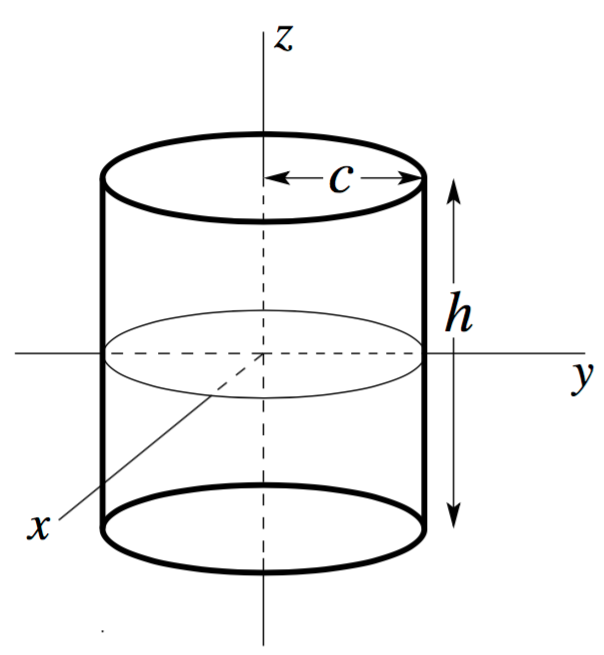
\includegraphics[scale=0.4]{10-point.png}
		\end{center}
		
	\end{problem}
	
	\begin{solution}
		\vfill
	\end{solution}
	\newpage
	
	
	\begin{problem}[Problem 2]
		Sketch the electric field lines for the electric quadrupole configuration shown in Figure 26-27. Explicitly indicate any points where the field is zero.
		\begin{center}
			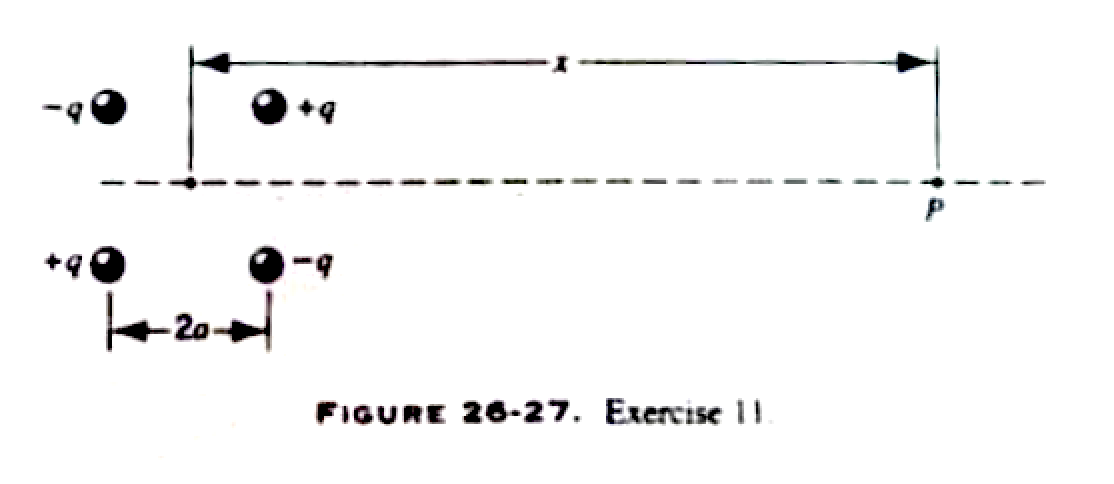
\includegraphics[scale=0.5]{26-27.png}
		\end{center}
		
		
	\end{problem}
	
	\begin{solution}
		\vfill
	\end{solution}
	\newpage
	
	
	\begin{problem}[HRK E26.16]
		A thin glass rod is bent into a semicircle of radius $r$. A charge $+q$ is uniformly distributed along the upper half and a charge $-q$ is uniformly distributed along the lower half, as shown in Fig. 26-28. Find the electric field $\vv{\textbf{E}}$ at $P$, the center of the semicircle.
		
		\begin{center}
			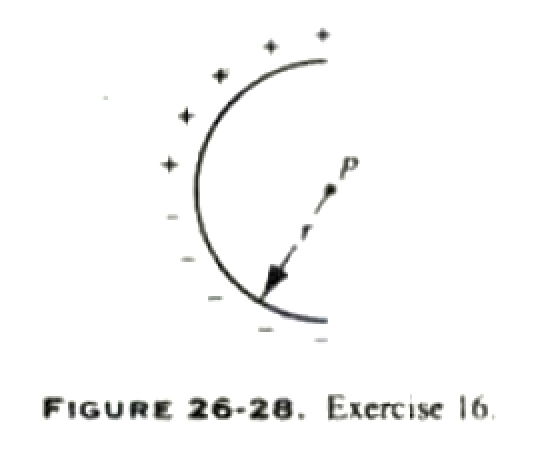
\includegraphics[scale=0.6]{26-28.png}
		\end{center}
			
	\end{problem}
	
	\begin{solution}
		\vfill
	\end{solution}
	\newpage
	
	
	\begin{problem}[HRK E26.18*]
		An insulating rod of length $L$ has charge $-q$ uniformly distributed along its length, as shown in Fig. 26-29.
		
		\begin{enumerate}
			\item[(a)] What is the linear charge density of the rod?
			\item[(b)] Find the electric field at point $P$ a distance $a$ from the end of the rod.
			\item[(c)] If $P$ were very far from the rod compared to $L$, the rod would look like a point charge. Show that your answer to $(b)$ reduces to the electric field of a point charge for $a \gg L$.
		\end{enumerate}
		
		\begin{center}
			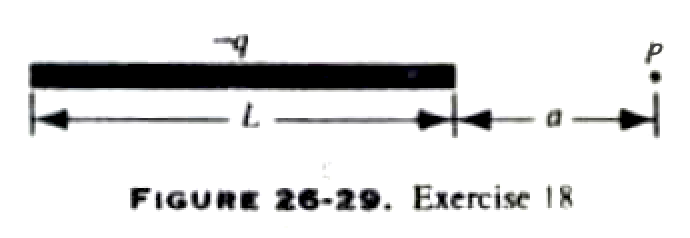
\includegraphics[scale=0.55]{26-29.png}
		\end{center}
	
		
	\end{problem}
	
	\begin{solution}
		\vfill
	\end{solution}
	\newpage
	
	\begin{problem}[HRK E36.40]
		Figure 26-36 shows a Thomson atom model of helium $(Z = 2)$. Two electrons, at rest, are embedded inside a uniform sphere of positive charge $2e$. Find the distance $d$ between the electrons so that the configuration is in static equilibrium.
		
		\begin{center}
			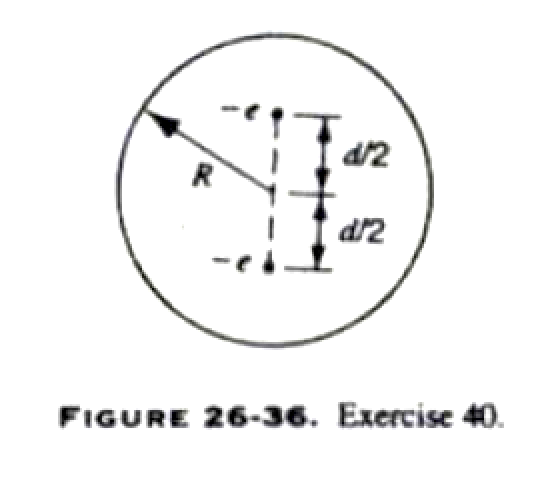
\includegraphics[scale=0.55]{26-36.png}
		\end{center}

	\end{problem}
	
	\begin{solution}
		\vfill
	\end{solution}
	\newpage
	
	\begin{problem}[HRK P26.7]
		A thin, non-conducting rod of finite length $L$ carries a uniform linear charge density $+\lambda$ on the top half and a uniform charge density $-\lambda$ on the bottom half; compare to Fig 26-6.
		
		\begin{enumerate}
			\item [(a)] Use a symmetry argument to determine the electric field at $P$ due to the rod.
			\item [(b)] Find $\vv{\textbf{E}}$ at $P$.
			\item [(c)] Take the limit of this expression for large $y$. How does it depend on $y$? What does this remind you of?
		\end{enumerate}
		
		\begin{center}
			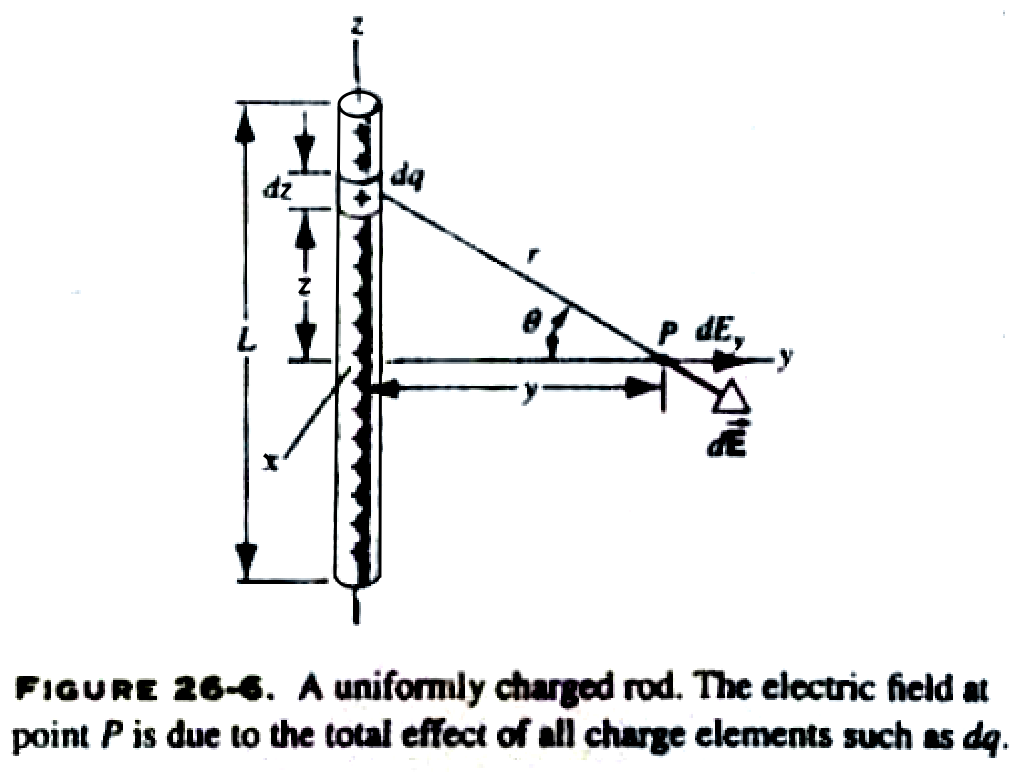
\includegraphics[scale=0.5]{26-6.png}
		\end{center}
		
	\end{problem}
	
	\begin{solution}
		\vfill
	\end{solution}
	
\end{document}